Un segment tree es una estructura en forma de \'arbol. Especificamente es un \'arbol binario, o sea, cada v\'ertice puede tener a lo m\'as dos hijos.

Cada nodo guarda un resultado precalculado para un rango del arreglo.  

Supongamos que nos dan un arreglo $a$ con los elementos $\{2, 3, 1, 6, 2, 1\}$ (comenzamos los \'indices desde el $1$ para mayor comodidad) y nos piden responder para cada consulta, la suma en el rango. Vamos a construir un segment tree para ese arreglo.

El valor correspondiente a la ra\'iz del \'arbol es la suma de los elementos del arreglo completo. El valor del hijo izquierdo de la ra\'iz es igual a la suma de los tres primeros elementos del arreglo. Igualmente, el valor del hijo derecho es igual a la suma de los tres \'ultimos elementos del arreglo.

En general, para cada nodo que no es hoja, si su rango es $[l, r]$, entonces el rango de su hijo izquierdo es $[l, m]$ y el de su hijo derecho es $[m+1, r]$, donde $m = \frac{l+r}{2}$.

Observe en la figura que el nodo correspondiente al rango $[1, 3]$ tiene un resultado igual a $6$ (que es la suma de los elementos en el rango) y que el resultado de su hijo izquierdo es $5$ y el de su hijo derecho es $1$.

Si el nodo es una hoja, su rango cubre solo un elemento del arreglo, por lo que su resultado puede calcularse inmediatamente y es igual al valor de dicho elemento.

\begin{minipage}{\columnwidth}
    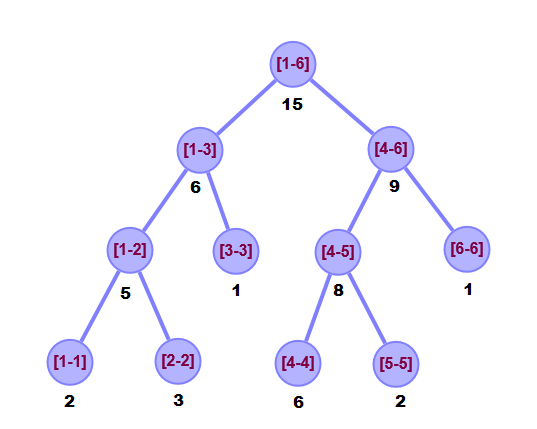
\includegraphics[width=\linewidth]{imag/segment_tree_suma.png}
    \label{example_sum}
\end{minipage}

Si nos pidieran calcular la suma de los elementos en el rango $[1, 5]$, lo cual es una consulta de rango, podemos obtener la res\-pues\-ta sin tener que recorrer todas las posiciones. Observe que podemos sumar los resultados de los nodos correspondientes a los rangos $[1, 3]$ y $[4, 5]$. Como vemos en la figura:

\begin{minipage}{\columnwidth}
    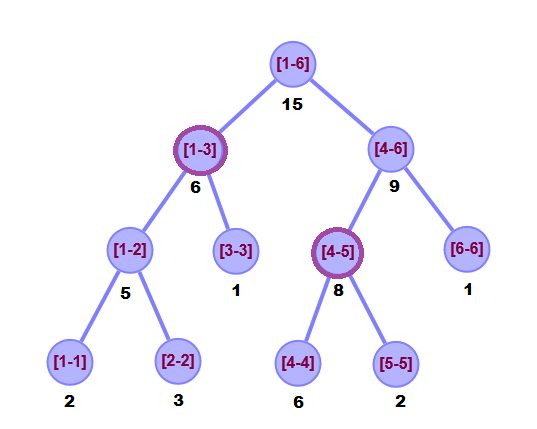
\includegraphics[width=\linewidth]{imag/segment_tree_query.png}
    \label{example_query}
\end{minipage}

Esa es la idea detr\'as de muchas estructuras de datos y especialmente del segment tree: precalculamos algunos valores que nos permiten luego obtener los resultados en menor tiempo. 

\hfill \break
\textit{?`Cu\'antos nodos puede tener un segment tree?}

Si construimos un segment tree para un arreglo de $n$ elementos, siendo $n$ igual a una potencia de $2$ ($n = 2^k$), el primer nivel del \'arbol, que es el de la ra\'iz, contiene un nodo ($2^0$ nodos); el segundo nivel tiene dos nodos ($2^1$ nodos), el tercer nivel tiene $2^2$ nodos y asi sucesivamente hasta el nivel que est\'a formado por las hojas, que son $2^k$.

El total de nodos ser\'a entonces:
$$ 2^0 + 2^1 + 2^2 + \cdots + 2^k = 2^{k+1} - 1 = 2 \cdot 2^k - 1$$

pero como $n = 2^k$, entonces el total de v\'ertices es $2 \cdot n-1$.

Si $n$ no fuera igual a una potencia de $2$, podemos agregar posiciones al final del arreglo hasta que $n$ sea igual a una potencia de $2$ y conseguir\'iamos el mismo resultado. 

\begin{property}
    La cantidad de v\'ertices m\'axima de un segment tree construido para un arreglo de largo $n$ es igual a $2\cdot n - 1$.
\end{property}

\hfill \break
\textit{?`Cu\'al es la altura m\'axima que puede tener un segment tree?}
Supongamos otra vez que construimos un segment tree para un arreglo de $n$ elementos, siendo $n$ igual a una potencia de $2$ ($n = 2^k$). El \'arbol tiene $k+1$ niveles (numerados desde $0$ hasta $k$). Pero como $n = 2^k$, entonces $k = \log_2(n)$; por lo que la altura del \'arbol ser\'a igual a $\log_2(n) + 1$.

\begin{property}
    La altura de un segment tree construido para un arreglo de largo $n$ es a lo m\'as $\log_2(n) + 1$.
\end{property}